\section{Design}
Sparkling Water is designed to be executed as a regular Spark application. It provides a way to initialize H2O services on each node in the Spark cluster and access data stored in data structures of Spark and H2O.

Since Sparkling Water is primarily designed as Spark application, it is launched
inside a Spark executor, which is created after application submission. At this
point, H2O starts services, including distributed K/V store and memory manager, and orchestrates them into a cloud. The topology of the created cloud matches the topology of the underlying Spark cluster exactly.

\begin{figure}[h]
	\centering
	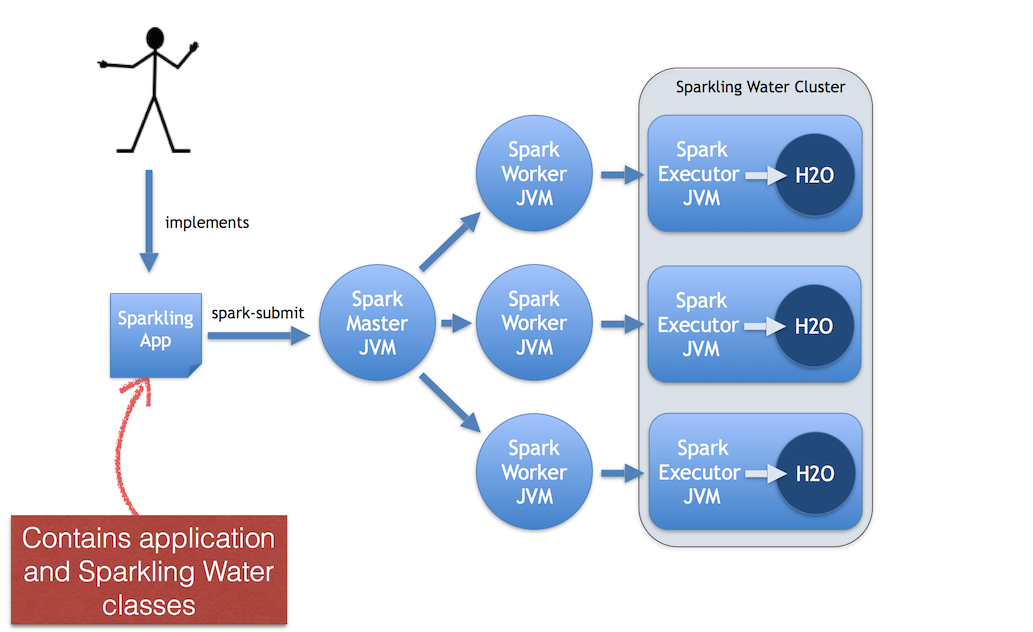
\includegraphics[width=\textwidth]{sw/images/Topology.png}
	\caption{Sparkling Water design. The scenario depicts deployment of Sparkling Water application to standalone Spark cluster.}
\end{figure}


\subsection{Data Sharing between Spark and H2O}

Sparkling Water enables transformation between different types of RDDs and H2O's H2OFrame, and vice versa.

When converting from H2OFrame to RDD, a wrapper is created around the H2O H2OFrame to provide an RDD-like API. In this case, no data is duplicated; instead, the data is served directly from then underlying H2OFrame.

Converting in the opposite direction (from RDD/DataFrame to H2OFrame) introduces data duplication, since it transfers data from RDD storage into H2OFrame. However, data stored in H2OFrame is heavily compressed and does not need to be preserved in RDD anymore.
\begin{figure}[h]
	\centering
	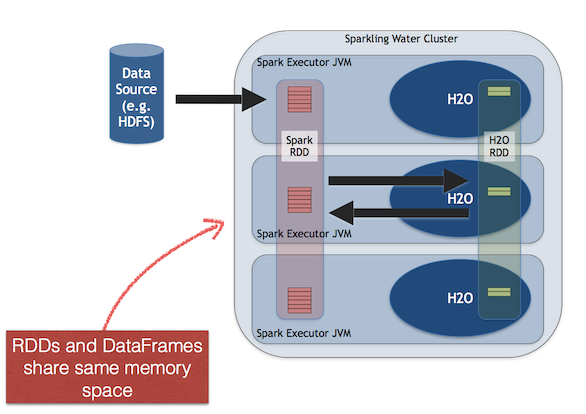
\includegraphics[width=0.7\textwidth]{sw/images/DataShare.png}
	\caption{Sharing between Spark and H2O inside an executor JVM.}
\end{figure}


\subsection{Provided Primitives}

The Sparkling Water provides several primitives (see Table~\ref{tab:primitives}). The first step before using H2O algorithms and data structures is to create and start \texttt{H2OContext} via \texttt{val hc = new H2OContext(sc).start()} call. The context holds information about running H2O services and exposes methods to transform data between Spark RDD/DataFrame and H2O Frame. The start of \texttt{H2OContext} involves distributed operation which contacts all accessible Spark executor nodes and initialize H2O services (KV store, RPC) inside executors' JVMs.

When \texttt{H2OContext} is running, H2O data structures and algorithms can be manipulated. The key data structure is \texttt{H2OFrame} which represents a distributed table composed of vectors. A new H2O frame can be created by:
\begin{itemize}
	\item loading a cluster local file\footnote{A file which is located on each node of the cluster.}:
\begin{lstlisting}[style=Scala]
val h2oFrame = new H2OFrame(new File("/data/iris.csv"))
\end{lstlisting}
	\item loading a file from HDFS/S3/S3N/S3A:
\begin{lstlisting}[style=Scala]
val h2oFrame = new H2OFrame(URI.create("hdfs://data/iris.csv"))
\end{lstlisting}
	\item transforming Spark RDD or DataFrame:
\begin{lstlisting}[style=Scala]
val h2oFrame = h2oContext.asH2OFrame(rdd)
\end{lstlisting}
	\item referencing existing H2O frame by its key
\begin{lstlisting}[style=Scala]
val h2oFrame = new H2OFrame("iris.hex")
\end{lstlisting}		
\end{itemize}


\begin{table}
\centering
\begin{tabularx}{\textwidth}{l l p{5.2cm}}
\toprule
Concept & API Representation & Description \\
\midrule
H2O context & \texttt{H2OContext}\footnote{Fullname of class is \texttt{org.apache.spark.h2o.H2OContext}} & Holds
H2O state and provides primitives to publish \texttt{RDD} as \texttt{H2OFrame} and
vice versa. It follows design principles of Spark primitives such as
\texttt{SparkContext} or \texttt{SQLContext} \\  \addlinespace

H2O entry point & \texttt{H2O}\footnote{Fullname of class is \texttt{water.H2Ot}} & Represents the entry point for accessing
H2O services. It holds information about running H2O services including a list of
nodes and the status of distributed K/V datastore. \\  \addlinespace

H2O Frame & \texttt{H2OFrame}\footnote{Fullname of class is \texttt{water.fvec.H2OFrame}} & A data structure that
represents a table of values. The table is column-based and provides column and
row accessors. \\  \addlinespace

H2O Algorithm & package \texttt{hex} & Represents the H2O machine learning
algorithms library, including DeepLearning, GBM, GLM, RandomForest and other
algorithms. \\

\bottomrule
\end{tabularx}
\caption{Sparkling Water primitives}
\label{tab:primitives}
\end{table}

When \texttt{H2OContext} is running any H2O algorithm can be called. Most of provided algorithms are located in the package \texttt{hex}. The call of an algorithm is composed of two step:

\begin{itemize}
	\item parameters specification:
\begin{lstlisting}[style=Scala]
val train: H2OFrame = new H2OFrame(new File("prostate.csv"))
val gbmParams = new GBMParameters()
gbmParams._train = train
gbmParams._response_column = 'CAPSULE
gbmParams._ntrees = 10
\end{lstlisting}

	\item creating model builder and launching computation. The \texttt{trainModel} method is non-blocking and returns a job which represents computation.
\begin{lstlisting}[style=Scala]
val gbmModel = new GBM(gbmParams).trainModel.get
\end{lstlisting}
\end{itemize}


